\lecture{23}{2024-12-23}{Famille Orthogonales}{}

\begin{parag}{Familles orthogonales}
    \begin{definition}
        Une famille $(\vec{u}_1, \dots, \vec{u}_k)$ de vecteurs $\mathbb{R}^n$ est \textcolor{red}{orthogonale} si $\vec{u}_i \perp \vec{u_j}$ pour tout $i \neq j$. Cette famille est orthonormée si de plus $||\vec{u}_i|| = 1$ pour tout $i$.
    \end{definition}
    \begin{subparag}{Rappel}
        \begin{enumerate}
            \item Deux vecteurs $\vec{u}$ et $\vec{v}$ de $\mathbb{R}^n$ sont \textcolor{red}{orthogonaux} si leur produit scalaire est nul
            \begin{formule}
            \[\vec{u}\cdot \vec{v} = 0\]
            \end{formule}
            \item Par distributivité du produit scalaire, $\vec{u}\perp\vec{a}$ et $\vec{u} \perp \vec{b}$ implique que
            $\vec{u} \perp Vect\{\vec{a}, \vec{b}\}$
        \end{enumerate}
        \begin{theoreme}
            Une famille orthogonale de vecteurs non nuls est libres
        \end{theoreme}
    \end{subparag}
\end{parag}
\begin{parag}{Coordonnées dans une base orthogonale}
    Soit $W$ un sous-espace de $\mathbb{R}^n$ et $(\vec{u}_1, \dots, \vec{u}_k)$ une base \textcolor{red}{orthogonale} de $W$.
    \begin{theoreme}
        Pour tout vecteurs $\vec{w}\in W$, on a $\vec{w} = \alpha_1\vec{u_1} + \cdots + \alpha_k\vec{u_k}$ et
        \[\alpha_j = \frac{\vec{w}\cdot\vec{u_j}}{||\vec{u_j}||^2}\]
    \end{theoreme}
    \begin{subparag}{Exemple}
        On construit une base orthogonale de $\mathbb{R}^3$ en commençant avec le plan d'équation $2x -3y + z = 0$.
        \\
        La méthode de Gausse nous fournit une base, par exemple, quitte à amplifier pour éviter des fractions, $\vec{b_1} = \begin{pmatrix}
            3\\2\\1
        \end{pmatrix} $ et $\vec{b_2} = \begin{pmatrix}
            -1 \\ 0 \\ 2
        \end{pmatrix}$.
        \\
        Or, ces deux vecteurs ne sont pas orthogonaux. Pour trouver un vecteurs de $W$ orthogonal à $\vec{b_1}$, je peux par exemple le choisir de la forme $\begin{pmatrix}
            -2 \\ 3 \\ c
        \end{pmatrix}$, le produit scalaire avec $\vec{b_1}$ vaut bien zéro, mais il faut encore que $c = 13$ pour que l'équation du play $W$ soit satisfaite. Ainsi on obtient une base orthogonale de $W$ avec 
        \[\vec{b_1} = \begin{pmatrix}
            3 \\ 2 \\ 0
        \end{pmatrix}\; \; \vec{b_2} = \begin{pmatrix}
            -2 \\ 3 \\ 13
        \end{pmatrix}\]
        On y ajoute encore $\vec{b_3} = \begin{pmatrix}
            2 \\ -3 \\ 1
        \end{pmatrix} \in W^\perp$ pour avoir une famille orthogonale de $\mathbb{R}^3 $
        \\
        On a donc la famille ordonnée $\bmath = \left(\begin{pmatrix}
            3 \\ 2 \\ 0
        \end{pmatrix}, \begin{pmatrix}
            -2 \\ 3 \\ 13
        \end{pmatrix}, \begin{pmatrix}
            2 \\ -3 \\ 1
        \end{pmatrix}\right)$ est  une famille orthogonale de vecteurs non nuls de $\mathbb{R}^3$, elle en forme donc une base.
        \begin{framedremark}
            Ce qu'on fait ici c'est qu'on a un plan dans un espace et on y rajouter un vecteurs qui y est orthogonale pour pouvoir avoir accès à tout l'espace, c'est comme si on pouvait "\textit{translater}" le plan dans l'espace.
        \end{framedremark}
        On cherche maintenant $(\vec{u})_\bmath$ qui est donné par:
        \[\vec{u} = \begin{pmatrix}
            1 \\ 1 \\ -1
        \end{pmatrix}\]
        On calcule maintenant $\vec{u}\cdot \vec{b_1} = 5$, $\vec{u}\cdot\vec{b_2} = -12$ et finalement $\vec{u}\cdot \vec{b_3} = -2$.
        \begin{framedremark}
            C'est la même principe qu'en physique lorsqu'un fait des projection du genre $\vec{v}\cdot \hat{e_x}$, on prend la composant sur l'axe du vecteurs.
        \end{framedremark}
        Ensuite afin de pouvoir le récrire dans la base il faut aussi gerer la longueur par rapport au vecteurs $\vec{b_1}\dots$ qui ont leur propre longueur, il font donc faire le ratio ce qui nous force à calculer les normes. $||\vec{b_1}||^2 = 13,\; ||\vec{b_2}||^2 = 182, \; ||\vec{b_3}||^2 = 14$
        \\
        On a qu'utiliser le théorème vu au dessus:
        \[(\vec{u})_\bmath = \begin{pmatrix}
            5/13\\-12/182 \\
            -2/14
        \end{pmatrix} = \begin{pmatrix}
            5/13\\
            -6/91\\
            -1/7
        \end{pmatrix}\]
    \end{subparag}
    \begin{subparag}{schéma du prof}
    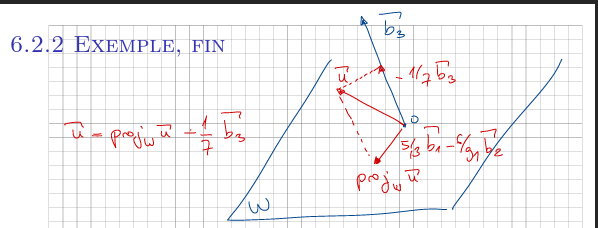
\includegraphics[scale = 0.75]{Algèbre linéaire/Screenshot 2024-12-04 101913.png}
    
    \end{subparag}
    \begin{framedremark}
        Ce qu'on fait ici c'est prendre le plan $\mathbb{R}^3$ à partir d'une base et donc on prend trois vecteurs pour couvrire tout l'espace. Mais attention à la consigne qui pourrait seulement demander le plan dans une famille de vecteurs orthogonale
    \end{framedremark}
\end{parag}

\begin{parag}{Matrice orthogonales}
    \begin{theoreme}
        Les colonnes d'une matrice $U$ de taille $m\times n$ sont orthonormées si et seulement si $U^TU = I_n$
    \end{theoreme}
    \begin{framedremark}
        ATTENTION, la réciproque ne marche pas $UU^T \neq I_n$ ça ne marche pas du tout
    \end{framedremark}
    \begin{subparag}{Preuve}
        Si $U = (\vec{u}_1, \dots, \vec{u}_n)$, alors le coefficient $(i, j)$ de la matrice $U^TU$ est exactement $\vec{u_i}^T\vec{u}_j = \vec{u}_i\vec{u}_j$. 
    \end{subparag}
    \begin{definition}
        Une matrice \textcolor{red}{carrée} $U$ est \textcolor{red}{orthogonale} si $U^TU = I_n$. Autrement dit $U^{-1} = U^T \Leftrightarrow$ colonnes (et lignes!) de $U$ sont orthonormées.
    \end{definition}
    Une matrice orthogonale représente un transformation linéaire qui préserve les distantes et l'orthogonalité (c'est donc une \textcolor{red}{isométrie} de $\mathbb{R}^n$, par exemple une rotation ou une symétrie)
\end{parag}

\begin{parag}{Préservation des longueurs}
    \begin{theoreme}
        Soit $U$ une matrice orthogonale. Alors
        \begin{itemize}
            \item $||U\vec{x}|| = ||\vec{x}||$ pour tout $\vec{x} \in \mathbb{R}^n$
            \item $U\vec{x}\cdot U\vec{y} = \vec{x}\cdot \vec{y}$
            \item $U\vec{x} \perp U\vec{y} \Leftrightarrow \vec{x}\perp \vec{y}$
        \end{itemize}
    \end{theoreme}
    \begin{subparag}{Problème technique}
        J'ai eu un problème avec overleaf donc j'ai pas pu écrire pendant le cours donc j'ai écrir un peu que les théorèmes et moins les exemples
    \end{subparag}
\end{parag}

\begin{parag}{ATTENTION}
    Si $U$ est orthogonale, alors aussi $UU^T = I_n$ Mais
    \begin{itemize}
        \item si $A$ est carrée avec $A^TA$ diagonale, $AA^T$ n'est pas diagonale en général
        \item Si $A$ n'est pas carrée avec $AA^T = I_n$, alors $A^TA \neq I_m$ en général
    \end{itemize}
\end{parag}
\begin{parag}{Projection orthogonale}
    Soit $W$ un sous-espace de $\mathbb{R}^n$ dont on dispose d'une base orthogonale $(\vec{u_1}, \dots, \vec{u}_k)$\\
    Pour $\vec{y} \in \mathbb{R}^n$ on cherche :
    \begin{itemize}
        \item Le vecteurs $\hat{y}\in W$ tel que
        \item le vecteur $\vec{z} = \vec{y}-\hat{y}$ est perpendiculaire à $W$.
    \end{itemize}
    \begin{theoreme}
        Tout vecteurs $\vec{y}$ de $\mathbb{R}^n$ s'écrit de manière unique $\vec{y} = \hat{y}+\vec{z}$ où $\hat{y}\in W$ et $\vec{z}\in W^\perp$
    \end{theoreme}
    \begin{subparag}{Remarque personelle}
        Ce qu'on voit ici c'est qu'il suffit de prendre un vecteurs qui se trouve dans le plan et de le "\textit{monter}" à la hauteur du vecteurs avec $\vec{z}$ qui lui est $\perp W$
    \end{subparag}
\end{parag}

\begin{parag}{Méthode}
    \begin{enumerate}
        \item Vérifier que la base de $W$ est orthogonale! tester toute les pairs $\vec{u_i}\cdot\vec{u}_j = 0$ pour tout les $i \neq j$
        \item Calculer les normes au carré des vecteurs de base $\vec{u_i}$
        \item Calculer les produits scalaires $\vec{y}\cdot\vec{u_i}$
        \item Calculer la projection
        \begin{formule}
            \[\hat{y} = \frac{\vec{y}\cdot \vec{u}_1}{||\vec{u_1}||^2}\vec{u_1} + \cdots + \frac{\vec{y}\cdot\vec{u}_k}{||\vec{u}_k||^2}\vec{u}_k\]
        \end{formule}
        \item Calculer $\vec{z} = \vec{y}-\hat{y}$ et \textcolor{red}{vérifier} que $\vec{z}\perp W$.
        \item \textbf{Remarque} Si $\vec{y} \in W$, alors $\hat{y} = \vec{y}$ et $\vec{z} = \vec{0}$
    \end{enumerate}
\end{parag}
\begin{parag}{Projection, cas d'une base orthonormée}
    Soit $(\vec{u_1}, \dots, \vec{u}_k)$ une base \textcolor{red}{orthonormée} de $W$, alors tous les $\vec{u_i}$ sont unitaires et:
    \begin{align*}
        \text{proj}_w\vec{y} &= (\vec{y}\cdot\vec{u}_1)\vec{u}_1 + \cdots +(\vec{y}\cdot\vec{u}_k)\vec{u}_k\\
        &= (\vec{u}_1^T\vec{y})\vec{u_1} + \cdots + (\vec{u}_k^T\vec{y})\vec{u}_k\\
        &= U\begin{pmatrix}
            \vec{u_1}^T\vec{y}\\
            \vdots\\
            \vec{u}_k^T\vec{y}
        \end{pmatrix} = UU^T\vec{y}
    \end{align*}

    \begin{theoreme}
        Soit $U$ la matrice dont les colonnes sont les vecteurs $\vec{u}_1, \dots, \vec{u}_k$ d'une base \textcolor{red}{orthonormée} de $W$. Alors:

        \begin{formule}
            \[\text{proj}_W\vec{y} = UU^T\vec{y}\]
        \end{formule}
    \end{theoreme}
\end{parag}
\begin{parag}{Approximation quadratique}
    La distance minimale entre un vecteurs $\vec{y}$ et un sous-espace $W$ de $\mathbb{R}^n$ est réalisée par $\vec{z} = \vec{y} - \text{proj}\vec{y}$
    \begin{theoreme}
        Pour tout $\vec{w} \in W$ on a $||\vec{y} - \vec{w}|| \geq ||\vec{y} - \text{proj}_W\vec{y}||$
    \end{theoreme}
    On appelle ce vecteurs $\hat{y}$ la meilleure approximation quadratique de $\vec{y}$ dans $W$ dans le sens où elle minimise le carré de la distance qui est calculée par la somme des carrées des coordonnées.
    \begin{subparag}{Idée de la preuve}
            L'idée est d'écrire un vecteurs $\vec{w}$ de $W$ de manière compliquée $\vec{w} = \hat{y} + (\vec{w} - \hat{y})$ afin de diviser en deux parti le vecteurs une qui est dans $W^\perp$ et l'autre dans $W$.
    \end{subparag}
\end{parag}

\begin{parag}{Le procédé de Gram Schmidt}
    \begin{itemize}
        \item \textbf{But} Trouver une base orthogonale ou rthonormée d'un sous-espace $W$ de $\mathbb{R}^n$
        \item \textbf{Idée} Utiliser de manière inductive les projections orthogonales. On considère dans $\mathbb{R}^4$ l'hyperplan $W$ donnée par l'équation
        \[x_1 + 2x_2 + x_3 + x_4 = 0\]
    \end{itemize}
    \begin{enumerate}
        \item On cherche d'abord une base, par exemple celle faite avec la méthode de gausse:
        \[\bmath = \left(\begin{pmatrix}
            -2 \\ 1 \\ 0 \\ 0
        \end{pmatrix}, \begin{pmatrix}
            -1 \\ 0  \\ 1 \\ 0
        \end{pmatrix}, \begin{pmatrix}
            -1 \\ 0 \\ 0 \\ 1
        \end{pmatrix}\right)\]
        on note les vecteurs $\vec{b_1}, \vec{b_2}, \vec{b_3}$
        \item On garde le premier vecteurs intacte et on va construire les autres vecteurs en fonction de celui la et donc
        \[\vec{c_1} = \vec{b_1}\]
        On projette $\vec{b_2}$ sur $Vect\{\vec{c_1}\}$ et on choisira $\vec{c_2} = \vec{b_2} - \hat{b_2}$.
        \item proj$_{Vect\{\vec{b_1}\}}\hat{b}_2 = \frac{\vec{b_1}\cdot\vec{b_2}}{||\vec{b_1}||^2}\vec{b_1} = \frac{2}{5}\vec{b_1} = \begin{pmatrix}
            -4/5\\2/5\\ 0\\0 
        \end{pmatrix}$
        \\
        On change $\vec{b_2}$ pour le rendre orthogonal à $\vec{c_1}$ :\\
        Et donc $\vec{c_2} = \vec{b_2}-\hat{b_2} = \begin{pmatrix}
            -1/5\\ -2/5 \\ 1 \\ 0
        \end{pmatrix}$
        \end{enumerate}
        Maintenant que nous avons une base orthogonale du plan $V = Vect\{\vec{b_1}, \vec{b_2}\}$, à savoir $(\vec{c_1}, \vec{c_2}$, les formules de projection sont à notre disposition pour calculer $\hat{b}_3 = \text{proj}_V\vec{b}_3$ et $\vec{c_3} = \vec{b_3} - \hat{b}_3$, où $\vec{b_3} = \begin{pmatrix}
            -1 \\ 0 \\ 0 \\ 1
        \end{pmatrix}$
        \\
        On cherche maintenant $\hat{b}_3 = \frac{\vec{b}_3 \cdot \vec{c}_1}{||\vec{c}_1||^2}\vec{c_1} + \frac{\vec{b}_3 \cdot \vec{c_2}}{||\vec{c_2}||^2}\cdot\vec{c_2} = \cdots = \begin{pmatrix}
            -5/6 \\ 1/3 \\ 1/6 \\0
        \end{pmatrix}$
        \\ Et donc:
        \[\vec{c_3} = \vec{b_3} - \hat{b}_3 = \begin{pmatrix}
            -1/6 \\ -1/3 \\ -1/6 \\ 1
        \end{pmatrix}\]
        Nous avons ainsi construire une base orthogonale $\cmath = (\vec{c_1}, \vec{c_2}, \vec{c}_3)$ de $W$. elle a les propriétés suivantes:
        \begin{itemize}
            \item Le vecteur $\vec{c_1} = \vec{b_1}$
            \item Le vecteurs $\vec{c_k}$ est combinaison linéaire des vecteurs $\vec{b_1}, \dots, \vec{b_k}$, en particulier c'est un vecteurs de $W$.
        \end{itemize}
\end{parag}
